\def\year{2020}\relax
%File: formatting-instruction.tex
\documentclass[letterpaper]{article} % DO NOT CHANGE THIS
\usepackage{aaai20}  % DO NOT CHANGE THIS
\usepackage{times}  % DO NOT CHANGE THIS
\usepackage{helvet} % DO NOT CHANGE THIS
\usepackage{courier}  % DO NOT CHANGE THIS
\usepackage[hyphens]{url}  % DO NOT CHANGE THIS
\usepackage{graphicx} % DO NOT CHANGE THIS
\urlstyle{rm} % DO NOT CHANGE THIS
\def\UrlFont{\rm}  % DO NOT CHANGE THIS
\usepackage{graphicx}  % DO NOT CHANGE THIS
\frenchspacing  % DO NOT CHANGE THIS
\setlength{\pdfpagewidth}{8.5in}  % DO NOT CHANGE THIS
\setlength{\pdfpageheight}{11in}  % DO NOT CHANGE THIS
%\usepackage[UTF8]{ctex}
\usepackage{booktabs} %table topline,midline,bottomline
\usepackage{algorithm}
\usepackage{algorithmicx}
%\nocopyright
%PDF Info Is REQUIRED.
% For /Author, add all authors within the parentheses, separated by commas. No accents or commands.
% For /Title, add Title in Mixed Case. No accents or commands. Retain the parentheses.
 \pdfinfo{
/Title (Synthesis of Registered Brain Multimodal MRI with Lesions)
/Author (Yili Qu,Wanqi Su,Chufu Deng,Ying Wang,Yutong Lu,Zhiguang Chen,Nong Xiao)
} %Leave this	
% /Title ()
% Put your actual complete title (no codes, scripts, shortcuts, or LaTeX commands) within the parentheses in mixed case
% Leave the space between \Title and the beginning parenthesis alone
% /Author ()
% Put your actual complete list of authors (no codes, scripts, shortcuts, or LaTeX commands) within the parentheses in mixed case. 
% Each author should be only by a comma. If the name contains accents, remove them. If there are any LaTeX commands, 
% remove them. 

% DISALLOWED PACKAGES
% \usepackage{authblk} -- This package is specifically forbidden
% \usepackage{balance} -- This package is specifically forbidden
% \usepackage{caption} -- This package is specifically forbidden
% \usepackage{color (if used in text)
% \usepackage{CJK} -- This package is specifically forbidden
% \usepackage{float} -- This package is specifically forbidden
% \usepackage{flushend} -- This package is specifically forbidden
% \usepackage{fontenc} -- This package is specifically forbidden
% \usepackage{fullpage} -- This package is specifically forbidden
% \usepackage{geometry} -- This package is specifically forbidden
% \usepackage{grffile} -- This package is specifically forbidden
% \usepackage{hyperref} -- This package is specifically forbidden
% \usepackage{navigator} -- This package is specifically forbidden
% (or any other package that embeds links such as navigator or hyperref)
% \indentfirst} -- This package is specifically forbidden
% \layout} -- This package is specifically forbidden
% \multicol} -- This package is specifically forbidden
% \nameref} -- This package is specifically forbidden
% \natbib} -- This package is specifically forbidden -- use the following workaround:
% \usepackage{savetrees} -- This package is specifically forbidden
% \usepackage{setspace} -- This package is specifically forbidden
% \usepackage{stfloats} -- This package is specifically forbidden
% \usepackage{tabu} -- This package is specifically forbidden
% \usepackage{titlesec} -- This package is specifically forbidden
% \usepackage{tocbibind} -- This package is specifically forbidden
% \usepackage{ulem} -- This package is specifically forbidden
% \usepackage{wrapfig} -- This package is specifically forbidden
% DISALLOWED COMMANDS
% \nocopyright -- Your paper will not be published if you use this command
% \addtolength -- This command may not be used
% \balance -- This command may not be used
% \baselinestretch -- Your paper will not be published if you use this command
% \clearpage -- No page breaks of any kind may be used for the final version of your paper
% \columnsep -- This command may not be used
% \newpage -- No page breaks of any kind may be used for the final version of your paper
% \pagebreak -- No page breaks of any kind may be used for the final version of your paperr
% \pagestyle -- This command may not be used
% \tiny -- This is not an acceptable font size.
% \vspace{- -- No negative value may be used in proximity of a caption, figure, table, section, subsection, subsubsection, or reference
% \vskip{- -- No negative value may be used to alter spacing above or below a caption, figure, table, section, subsection, subsubsection, or reference

\setcounter{secnumdepth}{2} %May be changed to 1 or 2 if section numbers are desired.

% The file aaai20.sty is the style file for AAAI Press 
% proceedings, working notes, and technical reports.
%
\setlength\titlebox{2.5in} % If your paper contains an overfull \vbox too high warning at the beginning of the document, use this
% command to correct it. You may not alter the value below 2.5 in
\title{Synthesis of Registered Brain Multimodal MRI with Lesions}
%Your title must be in mixed case, not sentence case. 
% That means all verbs (including short verbs like be, is, using,and go), 
% nouns, adverbs, adjectives should be capitalized, including both words in hyphenated terms, while
% articles, conjunctions, and prepositions are lower case unless they
% directly follow a colon or long dash
\author{\Large \textbf{Yili Qu,Wanqi Su,Chufu Deng,}\\ \Large \textbf{Ying Wang,Yutong Lu,Nong Xiao,Zhiguang Chen}\\  % All authors must be in the same font size and format. Use \Large and \textbf to achieve this result when breaking a line
 %If you have multiple authors and multiple affiliations
% use superscripts in text and roman font to identify them. For example, Sunil Issar,\textsuperscript{\rm 2} J. Scott Penberthy\textsuperscript{\rm 3} George Ferguson,\textsuperscript{\rm 4} Hans Guesgen\textsuperscript{\rm 5}. Note that the comma should be placed BEFORE the superscript for optimum readability
School of Data and Computer Science\\ Sun Yet-Sen University\\	
quyli@mail2.sysu.edu.cn% email address must be in roman text type, not monospace or sans serif
}
\begin{document}

\maketitle

\begin{abstract}
In a large number of data-driven medical images intelligent processing tasks, the collection and acquisition of medical image data is very difficult, especially the registered multimodal medical images data. Synthetic medical image data can well alleviate the problem of insufficient data. In this paper, based on the unsupervised conditional GAN model, we achieve the generation of registered multimodal medical images from random normal distribution matrix and corresponding lesion information can be efficiently generated based on the freely selected lesion label. We conducted a number of validation experiments on BRATS2015 to verify that our synthetic MRI can be used as pre-trained data or enhanced data in medical image intelligent processing tasks, and can greatly improve the generalization ability of the model.
\end{abstract}
	
\section{Introduction}
Magnetic resonance imaging (MRI) is a common medical image that can have multiple modalities depending on imaging parameters, such as T1, T2, T1c and so on. Different modalities have different reference values for doctors. To make accurate judgments, doctors often need multiple modal images to compare with each other. In the training and learning of medical image intelligent processing tasks, we often expect to obtain more modal images, such as medical image processing tasks based on Convolutional Neural Networks (CNN)\cite{86krizhevsky2012imagenet} or Generative Adversarial Networks (GAN)\cite{25goodfellow2014generative}. 

When obtaining different modalities from the same part of the same patient  through different imaging techniques, these modalities are considered to be registered if the imaging position and the viewing angle are identical.  Compared with unimodal data, the registered multimodal image data can provide more information, can support more complex application scenarios, meet the training data requirements of deep neural networks, and help to provide  intelligent diagnostic services more efficient and more reliable. For doctors, it takes longer to acquire images of different modalities and requires patient patience. For researchers of medical image intelligent processing tasks, multimodal MRI datasets are scarce, and the collection is very difficult, especially rare disease data, and the registered data is even rarer, which makes many training tasks impossible. Therefore, the application of image synthesis technology to extend datasets, translate existing unimodal images to registered multimodal images, generate registered multimodal images from random noise, has a wide range of uses and far-reaching significance.

Some studies explored cross-modal medical images translation prior to GAN by using graph dictionary mapping\cite{22burgos2015robust}, sparse coding\cite{33huang2017simultaneous},\cite{34vemulapalli2015unsupervised}, and CNN\cite{36vannguyen2015crossdomain}. Since then, many studies used GAN to generate higher quality translation results\cite{1zhao2018modular},\cite{5liang2018generative},\cite{6zhu2017unpaired},\cite{13choi2018stargan:}. Owe to the powerful capabilities of GAN, it has become the mainstream to achieve multimodal medical image translation\cite{2zhang2018translating},\cite{20nie2017medical},\cite{35osokin2017gans},\cite{36vannguyen2015crossdomain},\cite{40kamnitsas2017unsupervised}. The general translation is based on paired data, some studies have also learned from unpaired cross-modal data\cite{2zhang2018translating}. Recent studies have realized brain MRI to CT image translation with pixel-to-pixel GAN\cite{20nie2017medical},\cite{40kamnitsas2017unsupervised}, retinal vascular annotation to image translation\cite{41costa2017towards}, CycleGAN-based\cite{6zhu2017unpaired} cardiac MRI to CT image translation and segmentation\cite{20nie2017medical}. For multimodal synthesis, \cite{84chartsias2018multimodal} implements MRI synthesis of multiple inputs multiple outputs, but requires registration for input multimodal data. Based on this, \cite{85joyce2017robust} improves and implements a missing or unregistered multi-input synthesis model that can perform MRI image synthesis from any subset of its inputs, but limits the output to a single modality and the model is not scalable. \cite{66miao2018dilated} has conducted in-depth research on medical image registration. \cite{4shin2018medical} applys GAN to synthesize brain tumor images for data enhancement and data anonymization, but additional training of anatomical segmentation networks is required, and the dataset is required to have lesion segmentation labels, so the model generalization ability is weak. \cite{41costa2017towards} studies the random generation of vascular annotation maps based on the idea of Variational Auto-Encoder (VAE)\cite{87kingma2014auto-encoding, 88rezende2014stochastic}, and then synthesizes color retinal images. In these current studies of medical image synthesis, most are two-modal translation\cite{2zhang2018translating},\cite{20nie2017medical},\cite{22burgos2015robust},\cite{34vemulapalli2015unsupervised},\cite{35osokin2017gans},\cite{36vannguyen2015crossdomain},\cite{40kamnitsas2017unsupervised}, and the study of multimodal translation is very rare\cite{84chartsias2018multimodal},\cite{85joyce2017robust},\cite{4shin2018medical}. Outside the field of medical image processing, the development of many-to-many translation has recently made progress\cite{1zhao2018modular},\cite{5liang2018generative},\cite{13choi2018stargan:},\cite{27isola2017image-to-image}.

At present, there are various problems in the research of medical image synthesis, such as the difficulty of expanding the number of modalities, the need to registered training data, relying on complex large networks, the inability to add or retain lesions, the inability to generate from random matrices, and the need of additional training data, etc. Moreover, the evaluation of synthetic data in most studies relies on the evaluation of artificial visual effects by experienced physicians, without objective quantitative evaluation. Therefore, we design a registered multimodal MRI generation scheme based on the Conditional Generative Adversarial Networks (CGAN)\cite{70mirza2014conditional}. With unsupervised learning method, training data do not need to be registered. Our solution can receive a random normal distribution as input to generate a set of labeled multimodal registration MRI. We perform multimodal brain MRI generation experiments with tumor segmentation labels on BRATS2015, and verify the effectiveness of lesion information and the availability of synthetic data in tumor lesion segmentation experiments. See the open source code for details. Specifically, our contribution is in the following three areas:

\begin{itemize}
	\item \textbf{Extraction and Random Generation of Structural Feature Maps}
	We propose an extraction method for anatomical features for medical images. Without additional anatomical segmentation labels or label extraction training, structural feature maps can be extracted directly from real images of arbitrary modalities ,and assist GAN to learn to generate more reasonable synthetic images. The extraction method can directly obtain the anatomical features of real images, and improve the quality of synthetic images without introducing additional parameters and computation overhead. We also train a structural feature map generator to generate structural feature maps from multidimensional normal distribution. The random generation method can generate rich and diverse structural feature maps indefinitely.
	\item \textbf{Synthesis of Registered Multimodal MRI with Lesion Label}
	based on input lesion labels during multimodal MRI synthesis. In training, no registration data is required, no additional label data is required except for the lesion label, the synthetic data is registered, and the random lesion label is the lesion label of the synthetic data. Our solution enables fast and easy construction of registered multimodal MRI datasets with label.
	\item \textbf{Objective Verification Method for Synthetic Data Availability}
	We construct datasets with different amount of synthetic and real data to train the lesion segmentor, and verify that the synthetic data can be used as pre-training data and enhanced data in the medical image intelligent processing tasks to improve the generalization ability of the model and improve the segmentation precision. Compared with the traditional subjective evaluation method of synthetic image quality, we present the availability of synthetic data in intelligent lesion processing tasks more objectively.
\end{itemize}


\section{Method}
\label{method}
We perform our scheme on multimodal brain MRI synthesis task, in which the synthetic lesion is tumors, the lesion label is a tumor segmentation label, and the lesion processing task is lesion segmentation. Our scheme does not limit the synthesis of human parts, lesion types, lesion processing tasks, specific modality and the number of modalities. We can easily apply this method to other similar tasks through the following example.
\subsection{Architecture}
\begin{figure}[t]
	\centering
	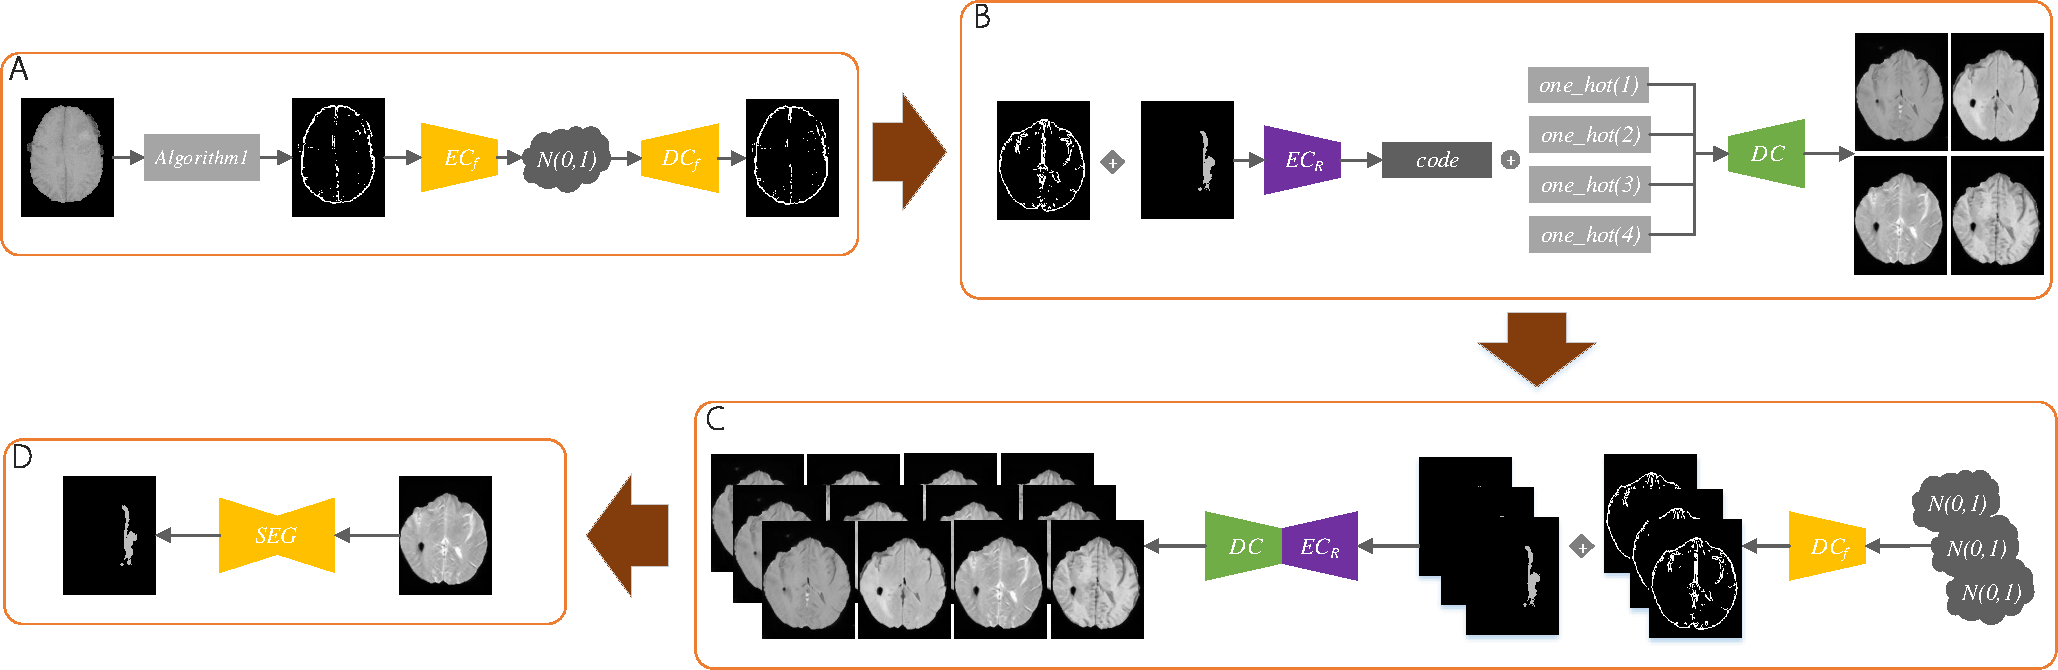
\includegraphics[width=0.98\columnwidth]{figures/architecture}
	\caption{Architecture.}
	\label{architecture}
\end{figure}
As shown in Fig.~\ref{architecture}, our scheme includes four main stages: structural feature map extraction and random generation, multimodal MRI generation, construction of synthetic datasets, and synthetic data availability verification.

In the structural feature map extraction and random generation stage, we will obtain a structural feature map generator that can generate structural feature maps from the random normal distribution matrix. Models we train at this stage includes a structural feature map encoder, a structural feature map decoder, a structural feature map discriminator, a code distribution discriminator and a structural feature mask generator.

In the multimodal MRI generation stage, we generate a conditional generator with input of structural feature maps, which can generate MRIs of different modalities according to different one-hot conditional vectors, and can add lesion labels on the structural feature maps to generate MRI has corresponding lesion information. At this stage, we train a structural feature map and lesion label fusion encoder, a lesion segmentor for each modality, an MRI encoder, an MRI decoder, an MRI discriminator and an MRI code discriminator.

In the stage of constructing the synthetic datasets, we use the model produced in the first two stages to generate a sufficient number of structural feature maps from the random normal distribution matrix and then randomly fuse with real lesion labels, and finally generate the registered multimodal MRI to construct synthetic datasets.

In the synthetic data availability verification stage, we train a lesion segmentor for each MRI modality based on real data, and perform segmentation ability tests on real dataset. Then these segmentors are used to perform segmentation tests on the synthetic data generated by different lesion generation guidance methods. In addition, we use datasets constructed from synthetic data and real data of different amounts to train the lesion segmentor. After training, the segmentation ability test is performed on the real dataset, and the test results are compared to verify the availability of the synthetic data in lesion segmentor training.

\subsection{Structural Feature Map Extraction Method}

Medical images generated directly from random noise by GAN are often difficult to train and difficult to generate real structural information. We call image that provide basic contour and structure information as structural feature map. For example, a retinal blood vessel distribution map can be regarded as a structural feature map of a retinal image\cite{41costa2017towards}. Structural feature maps can provide necessary basic guidance for the synthesis of medical images. For example, when synthesizing brain MRI, some studies obtain basic structural information from the brain segmentation label\cite{4shin2018medical}. However, common structural features such as retinal vascular maps and brain segmentation labels require additional data and training to extract structural features from the original image. To this end, we first design a method for extracting structural feature maps directly from brain MRI, which has the advantages of fast operation, no training, no additional data. 

In the traditional digital image processing methods, Roberts operator, Prewitt operator, Sobel operator, etc. are excellent edge detection operators. Sobel operator is often used in processing of brain medical images, and their convolution kernel parameters and calculation formula are as shown. As shown in Algorithm~\ref{alg:1}, We explore a method for further extracting structural feature maps from the edge detection maps generated by Sobel operator.
\begin{algorithm}
	\caption{Structural Feature Extraction}
	\label{alg:1}
	\begin{algorithmic}[1]
		\State Input a real image $x$,$beta$ is pixel threshold
		\State $f1 = reduce\_min(sobel(x))$
		\State $f2 = reduce\_max(sobel(x))$
		\State $f1 = mean(f1) - f1$
		\State $f2 = f2 - mean(f2)$
		\State $f1 = ones * (f1 > beta)$
		\State $f2 = ones * (f2 > beta)$
		\State $f = f1 + f2$
		\State $f = ones * (f > 0.)$
	\end{algorithmic}  
\end{algorithm}

In Algorithm~\ref{alg:1} we use Sobel operator to extract the horizontal and vertical edge detection maps from a real image, each perform reduce maximum and reduce minimum to obtain two edge detection fusion maps, each fusion map calculate the difference with average pixel value, the two difference maps are binarized according to the set pixel threshold, and the two binary images are summed and then completely binarized. The final result is the structural feature map we need.

\subsection{Training of Random Structural Feature Map Generation}

When generating the structural feature map, \cite{4shin2018medical} still needs to input the real modal image to get the generated structural feature map, which greatly reduces the diversity of generated data, and \cite{41costa2017towards} implements a method for generating retinal blood vessel distribution maps from multidimensional normal distribution. On the basis of this, we design a method for generating brain structural feature maps from random noise, which has better diversity and no additional data. 
Specifically, we design a hybrid network combining the characteristics of VAE and GAN. First, we encode the structural feature map extracted from real image into a mean matrix and a variance matrix through the VAE encoder, then fuse with a random normal distribution matrix to form an approximate normal distribution matrix, and gradually approach the standard normal distribution through the loss constraint. Then, we use VAE decoder to reconstruct the structural feature map from the approximate normal distribution matrix. The decoder is trained by self-supervised reconstruction loss of structural feature maps. For the constraint of approximate normal distribution matrix, we do not use the VAE encoder loss, but add a code distribution discriminator. The code distribution discriminator learns normal distribution matrix as a positive sample and latent feature matrix as a negative sample, and provides adversarial loss for encoder. Meanwhile, we use $L2$ regular loss to guide the mean matrix with a mean of 0 and the variance deviation matrix with a mean of 1. In addition, we use another discriminator to receive structural feature map extract from real MRI and randomly generated structural feature map for adversarial learning, so that the generated structural feature map becomes more and more realistic.
\begin{figure}
	\centering
	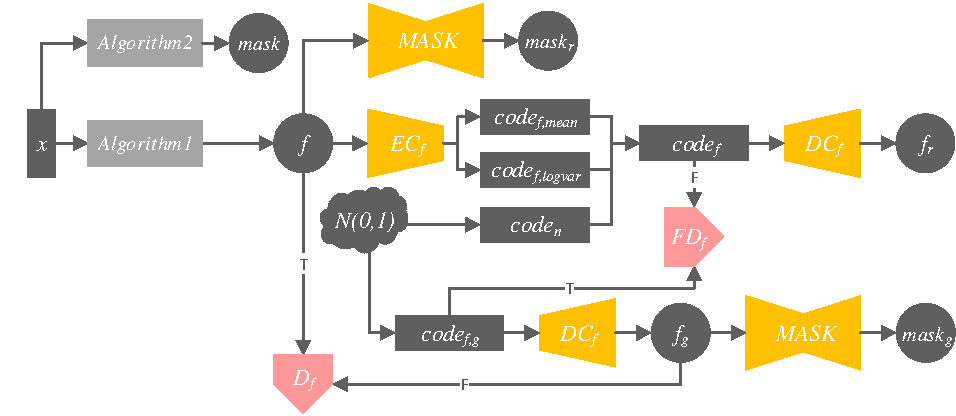
\includegraphics[width=0.98\columnwidth]{figures/feature_train}
	\caption{Training of Random Structural Feature Map Generation.}
	\label{feature_train}
\end{figure}

In order to prevent the generated brain MRI pixel area from exceeding the brain outline of the structural feature map, we train a generator $MASK$ that acquires the brain area mask from the brain structure feature map. The generator is synchronized with the  training of structural feature map generation. During training, the mask extracted by the real brain MRI$x$ through the mask extraction algorithm (Algorithm~\ref{alg:2}) is used as label data.
\begin{algorithm}
	\caption{Mask Extraction}
	\label{alg:2}
	\begin{algorithmic}[1]
		\State Input a real image $x$, $p$ is expanded pixel value
		\State $mask = 1.0 - ones * (x > 0.)$
		\State $shape = get\_shape(x)$
		\State $mask = resize(mask, size=[shape[1] + p, shape[2] + p])$
		\State $mask = crop\_padding(mask, crop\_length=p, crop\_width=p)$
	\end{algorithmic}  
\end{algorithm}

As shown in Fig.~\ref{feature_train}, the specific processing procedure for decoding the random structure feature map from standard normal distribution is as follows:
\begin{itemize}
	\item The structural feature map $f$ is obtained from real MRI$x$ using the structural feature extraction method, and the mask $mask$ is obtained by the mask extraction algorithm(Algorithm~\ref{alg:2});
	\item Encode $f$ with encoder $EC_f$ to get $code_{f,mean}$ and $code_{f,logvar}$, get a random noise $code_n$ from multidimensional normal distribution $\mathcal{N}(0,1^2)$ , the approximate normal distribution matrix is obtained from three codes $code_f=code_{f,mean}+exp(0.5*code_{f,logvar})*code_n$ ;
	\item Decode $code_f$ with decoder $DC_f$ to obtain the reconstructed structural feature map $f_r$;
	\item Use mask generator $MASK$ to extract mask $mask_r$ from $f$;
	\item Randomly generate a matrix $code_{f,g}$ that obeys normal distribution $\mathcal{N}(0,1^2)$;
	\item Decode $code_{f,g}$ with decoder $DC_f$ to get the generated random structure feature map $f_g$;
	\item Use mask generator $MASK$ to extract mask $mask_g$ from $f$;
	\item Structural feature discriminator $D_f$ identifies $f$ and $f_g$ respectively, identifying the former as true and the latter as false;
	\item Code distribution discriminator $FD_f$ discriminates between $code_f$ and $code_{f,g}$, respectively, identifying the former as false and the latter as true.
\end{itemize}

In training, we perform adversarial training through discriminator $D_f$ to make the structural feature map decoded by decoder more realistic. In addition, the adversarial training is performed by the feature discriminator $FD_f$, so that encoder $EC_f$ can encode structural feature map $f$ to standard normal distribution. The complete loss items are as follows, where $\omega_{i,j}$ is the weight of each loss item: 
\begin{itemize}
	\item \textbf{Discriminator Loss of Code Distribution } 
	\begin{center}
		$loss_{FD_f}=\Vert{FD_f(code_{f,g})-1}\Vert_{2}^{2}+\Vert{FD_f(code_f)}\Vert_{2}^{2}$
	\end{center}
	
	\item \textbf{Discriminator Loss of Structural Feature Map} 
	\begin{center}
		$loss_{D_f}=\Vert{D_f(f)-1}\Vert_{2}^{2}+\Vert{D_f(f_g )}\Vert_{2}^{2}$
	\end{center}
	
	\item \textbf{Adversarial Loss} 
	\begin{center}
		$loss_{G_f}=\Vert{FD_f(code_f)-1}\Vert_{2}^{2}+\Vert{D_f(f_g)-1}\Vert_{2}^{2}$
	\end{center}
	
	\item \textbf{Supervised Loss of Structural Feature Code Distribution} 
	\begin{center}
		$loss_{normal}=\Vert{mean(code_{f,mean})}\Vert_{2}^{2}+ \Vert{mean(exp(0.5*code_{f,logvar}))-1}\Vert_{2}^{2}$
	\end{center}
	where $mean()$ is a mean function.
	
	\item \textbf{Self-supervised Loss of Structural Feature Map and Mask} 
	\begin{center}
		$loss_{sv}=\Vert{f-f_r}\Vert_{2}^{2}+\Vert{f_r*mask}\Vert_{2}^{2}$
	\end{center}
	
	\item \textbf{Mask Generator Loss}
	\begin{center}
		$loss_{mask}=\Vert{mask-mask_r }\Vert_{2}^{2}+\Vert{f*mask_r}\Vert_{2}^{2}+\Vert{f_r*mask_r}\Vert_{2}^{2}+\Vert{f_g*mask_g}\Vert_{2}^{2}$
	\end{center}
\end{itemize}

\subsection{Real MRI reconstruction and translation training}
We perform MRI reconstruction and translation training on real MRI, using a set of MRI encoder, MRI decoder and MRI discriminator, as well as a set of lesion label generation components. All of the components of this training process will be described in the subsequent multimodal MRI generation training section, and the training process in this section is synchronized with the multimodal MRI generation training. We constrain each component to complete our assigned tasks during multimodal MRI generation by synchronous MRI reconstruction and translation training on real data. In addition, we also use a code discriminator to guide the consistency of the two training processes. The discriminator training process is shown in Fig.~\ref{train_D}

\begin{figure}
	\centering
	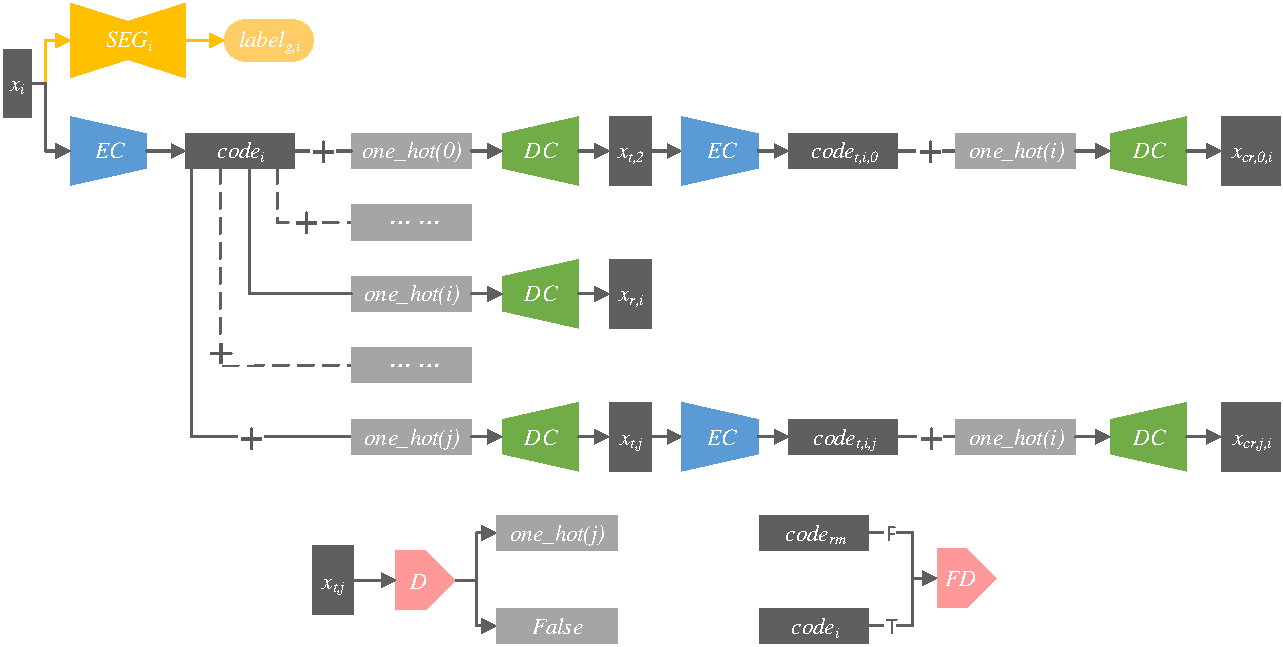
\includegraphics[width=0.98\columnwidth]{figures/trans_train}
	\caption{Auxiliary modality reconstruction and modality translation training.}
	\label{trans_train}
\end{figure}

As shown in Fig.~\ref{trans_train}, when the MRI is reconstructed and translated, the encoder encodes the real MRI $x_i$ of modality $i$ to obtain the semantic feature map $code_{i}$, then we connect it to different conditional vectors and decode all the modalities through the decoder. In cycle-reconstruction, we use encoder to re-encode all the obtained translation images, connect all the re-encoded semantic feature maps with the conditional vector of modality $i$, and finally decode them by decoder to get cycle-reconstruction image $x_{rc,j,i}$. 【】
In the above process, we use the lesion label $l_i$ of the original input modality $x_i$ as supervised label for the lesion generation training, and use lesion label generation components for $x_i$ to get $l_{r,i}$.

Our discriminator components are updated independently, and other components are updated through an optimizer. The loss items include the adversarial loss and category guidance loss provided by discriminator, self-supervised loss of MRI reconstruction, self-supervised loss of MRI cycle-reconstruction, consistency loss of MRI cycle-reconstruction, semantic consistency loss, and supervised loss of lesion generation. 

The detailed losses are as follows, where $x_{r,i}$ represents the MRI reconstruct from modality $i$, and $x_{t,j,i}$ refers to MRI of modality $i$ translated by modality $j$. $d_{t, j, i}$ and $c_{t, j, i}$ are the true/false discrimination and category discrimination results of the discriminator for $x_{t, i, j}$, $x_{cr,j,i}$ represents MRI that translate from modality $i$ to modality $j$ then translate back to modality $i$; $code_i$ represents the semantic feature map obtained from $x_i$ by encoder, $code_{t,i,j}$ represents the semantic feature map obtained from $x_{t,i,j}$ by encoder; $l_i$ represents the real lesion label of $x_i$, $l_{r,i}$ represents the lesion label generated by lesion label generation components from $x_i$ :

\begin{itemize}
	\item \textbf{discriminator loss}
	\begin{center}
		$loss_{D,assist}=\sum\limits_{j=0,j\neq i}\sum\limits_{i=0}(\Vert{d_{t,j,i}}\Vert_{2}^{2}+\Vert{c_{t,j,i}-i}\Vert_{2}^{2})$
	\end{center}
	
	\item \textbf{adversarial loss and category guidance loss}
	\begin{center}
		$loss_{G,assist}=\sum\limits_{j=0,j\neq i}\sum\limits_{i=0}(\Vert{d_{t,j,i}-1}\Vert_{2}^{2}+\Vert{c_{t,j,i}-i}\Vert_{2}^{2})$
	\end{center}
	
	\item \textbf{self-supervised loss of MRI reconstruction}
	\begin{center}
		$loss_{sv}=\sum\limits_{i=0}(\Vert{x_i-x_{r,i}}\Vert_{2}^{2})$
	\end{center}
	
	\item \textbf{self-supervised loss of MRI cycle-reconstruction}
	
	\begin{center}
		$loss_{cycle}=\sum\limits_{j=0,j\neq i}\sum\limits_{i=0}(\Vert{x_i-x_{cr,j,i}}\Vert_{2}^{2})$
	\end{center}
	
	\item \textbf{consistency loss of MRI cycle-reconstruction}
	\begin{center}
		$loss_{cycle,consistency}=\sum\limits_{k=0,k\neq j,k\neq i}\sum\limits_{j=0,j\neq i}\sum\limits_{i=0}(\Vert{x_{cr,j,i}-x_{cr,k,i}}\Vert_{2}^{2})$
	\end{center}
	
	\item \textbf{semantic consistency loss}
	\begin{center}
		$loss_{code,consistency}=\sum\limits_{j=0,j\neq i}\sum\limits_{i=0}(\Vert{code_i-code_{t,i,j}}\Vert_{2}^{2})$
	\end{center}
	
	\item \textbf{supervised loss of lesion generation}
	\begin{center}
		$loss_{sv,l}=\sum\limits_{i=0}\Vert{label_i-label_{r,i}}\Vert_{2}^{2}$
	\end{center}
	
\end{itemize}

\subsection{Fusion of structural feature maps and lesion segmentation labels}

When the structural feature map is fused with the lesion segmentation label, we first generate structural feature map $f_g$ from random standard normal distribution matrix, then randomly select the appropriate lesion segmentation label $label$, and then the lesion segmentation label containing $n$ categories is converted into a one-hot matrix $onehot_l$ of $n$ channels, and each channel corresponds to a segmentation category, the pixel value in each channel is 0 or 1. The pixel value of the same area as the corresponding category segmentation position is 1 and the rest is 0, so that each 1 pixel area is registered with each segmentation area in the segmentation label. Next, we calculate the weighted sum of each channel of $onehot_l$ with $f_g$, and get a new matrix that fuses the information of $f_g$ and $label$.

If the structural feature map $f'$ is extracted from the random MRI $x$, then the extracted structural features may contain tumor structure information, which may interfere with the tumor information in random label $l$ and affect the fusion generation MRI, so $f'$ needs to eliminate the tumor information before fusing with the random label $label$, and get the structural feature map $f$ without tumor information, so that the tumor information of the generated image is only derived from the label $label$. We generate a  mask without boundary expansion $mask_{l,x}$ for segmentation label $label_x$ of $x$ by the Algorithm~\ref{alg:2}, then we have $f=mask_{l,x}\times f'$.

Since the location of the randomly selected lesion may appear outside the brain contour of structural feature map, we need to use the Algorithm~\ref{alg:2} to obtain the brain region mask $mask$ of the structural feature map. If the product of $mask$ and the selected $label$ is 0, then the tumor label pixel is inside the brain contour of $mask$, which can be adopted, otherwise the $label$ needs to be re-selected.

\subsection{Multimodal MRI generation training}
\begin{figure}
	\centering
	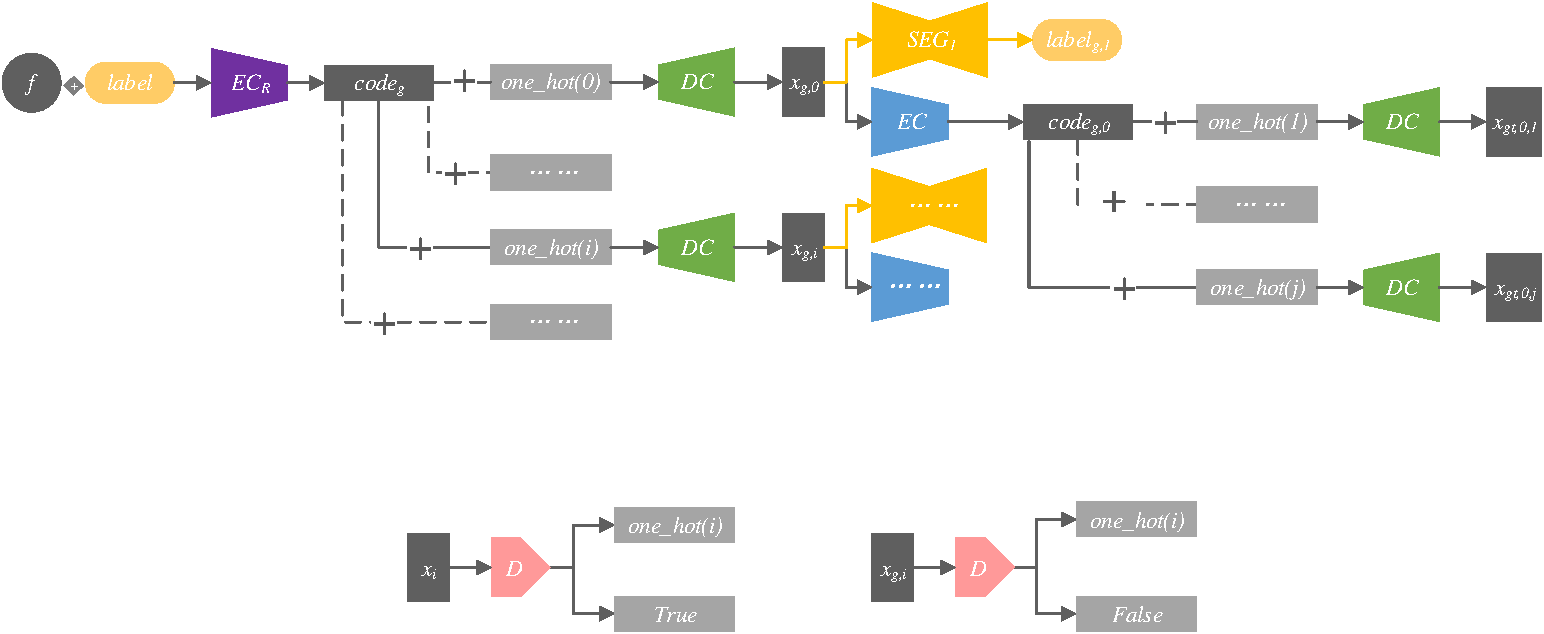
\includegraphics[width=0.98\columnwidth]{figures/mm_mri_generate}
	\caption{generation of Multimodal MRI.}
	\label{mm_mri_generate}
\end{figure}

\begin{figure}
	\centering
	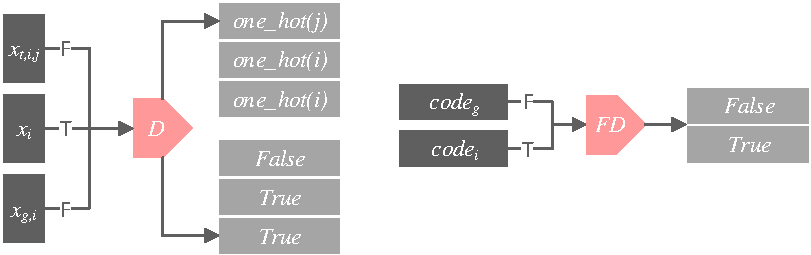
\includegraphics[width=0.8\columnwidth]{figures/D}
	\caption{reconstruction and translation training of real MRI and discriminator training during multimodal MRI generation training.}
	\label{train_D}
\end{figure}

We extract the structural feature map $f$ from the real MRI by the Algorithm~\ref{alg:1}, and randomly select the real lesion label $label$, and merge with the lesion segmentation label by the above fusion method. The fusion map contains basic anatomical information and lesion information of the target site. The multimodal MRI generated from the fusion map is easier to train than the multimodal MRI generated directly from random noise, and the generated MRI is more reasonable and realistic. The multimodal MRI generation process is shown in Fig.~\ref{mm_mri_generate}. First, we use a fusion map encoder to encode fusion map to obtain the semantic feature map. The semantic feature map is stacked with different conditional vectors and decodes by MRI decoder to obtains synthesis image of different modalities. We use adversarial loss and category guidance loss provided by MRI discriminator to constrain synthesis image to approximate real MRI. And images of each modalities are then encoded by MRI encoder to obtain semantic feature maps. These semantic feature maps are stacked with different conditional vectors and decoded by MRI decoder to realize the modal translation. We constrain the consistency of all semantic feature maps and translation images by loss, thus ensuring the mutual registration of generated multimodal MRI. In addition, we used a set of lesion label generation components to segment the tumor lesion segmentation labels from each synthetic MRI to ensure that the generated multimodal images have generated corresponding lesion content based on the input lesion label.

Our discriminator components are updated independently. The lesion label generation component is only trained and updated using real data in reconstruction and translation training, and is used in this section only to provide lesion generation guidance loss for MRI generation components. Other components are updated through an optimizer.

The specific loss items of the multimodal MRI generation process are as follows, where $d_{i}$ and $c_{i}$ are the rue/false discrimination and category discrimination of the discriminator $D(x_i)$, $d_{g, i}$,$c_{g,i}$ is the output of $D(x_{g,i})$; $x_{g,i}$ is the synthetic image of modality $i$, $x_{gt,j,i}$ is the translation image of the modality $i$ translated by synthetic image of modality $j$; $code_g$ is the semantic feature map obtained by fusion map encoder$EC_R$, $code_{g,i}$ is the semantic feature map encoded from $x_i$; $l$ is the input label, $l_{g,i}$ is the label obtained by lesion label generation component from $x_{g,i}$; $f$ is the input structural feature map, $f_{g,i}$ is the structural feature map extracted from $x_{g,i}$ by Algorithm~\ref{alg:1}
\begin{itemize}
	\item \textbf{true/false Discrimination loss of Discriminator}
	\begin{center}
		$loss_{D}=\sum\limits_{i=0}(\Vert{d_{i}-1}\Vert_{2}^{2}+\Vert{d_{g,i}}\Vert_{2}^{2})$
	\end{center}

	\item \textbf{modality Discrimination loss of Discriminator}
	\begin{center}
	$loss_{D,class}=\sum\limits_{i=0}(\Vert{c_{i}-i}\Vert_{2}^{2}+\Vert{c_{g,i}-i}\Vert_{2}^{2})$
	\end{center}

	\item \textbf{adversarial loss}
	\begin{center}
		$loss_{G}=\sum\limits_{i=0}(\Vert{d_{g,i}-1}\Vert_{2}^{2})$
	\end{center}
	
	\item \textbf{Modality category guidance loss}
	\begin{center}
		$loss_{G,class}=\sum\limits_{i=0}(\Vert{c_{g,i}-i}\Vert_{2}^{2})$
	\end{center}
	
	\item \textbf{Reconstruction self-supervised loss of input structural feature map}
	\begin{center}
		$loss_{sv,f}=\sum\limits_{i=0}(\Vert{f-f_{g,i}}\Vert_{2}^{2})$
	\end{center}
	
	\item \textbf{supervised loss of Lesion label generation }
	\begin{center}
		$loss_{sv,l}=\sum\limits_{i=0}(\Vert{label-label_{g,i}}\Vert_{2}^{2})$
	\end{center}
	
	\item \textbf{supervision loss of MRI registration}
	\begin{center}
		$loss_{trans}=\sum\limits_{j=0,j\neq i}\sum\limits_{i=0}(\Vert{x_{g,i}-x_{gt,j,i}}\Vert_{2}^{2})$
	\end{center}
	
	\item \textbf{semantic consistency loss}
	\begin{center}
		$loss_{trans,code}=\Vert{code_g-code_{g,i}}\Vert_{2}^{2}+\sum\limits_{j=0,j\neq i}\sum\limits_{i=0}(\Vert{code_{g,i}-code_{g,j}}\Vert_{2}^{2})$
	\end{center}
	
\end{itemize}

\subsection{Lesion label generation guidance method}
\label{label gen methods}
We design the following three lesion label generation components to provide guidance loss for lesion generation in multimodal MRI generation training:
\begin{itemize}
	\item \textbf{Single segmentor} 
	Each modality is segmented from synthetic MRI by a common complete segmentor to obtain the respective lesion label.
	\item \textbf{Single lesion encoder + multiple lesion decoders} 
	Different modality segmentors are combined by a common lesion encoder and different lesion decoders. 
	\item \textbf{multiple segmentors} 
	Each modality is segmented from synthetic MRI by a separate complete segmentor to obtain the respective lesion label.
\end{itemize}
The loss item of the above three schemes is consistent with the loss item described above, and each component of the three methods is only trained using supervised loss of lesion label generation in real MRI reconstruction and translation training.

\subsection{construction of synthetic datasets}
\label{make dataset}
As shown in Fig.~\ref{make_data}, we can generate any number of structural feature maps from randomly generated normal distribution matrix through the trained structural feature map decoder. Then, we randomly scaled, rotated, translated, flipped, etc. the original set of labels to get a random lesion label set. We then fuse the randomly generated structural feature map with the randomly selected lesion label from the random lesion label set. Similarly, we can select suitable random lesion labels by obtaining mask from structural feature map through the mask generator $MASK$. Similarly, we can select suitable random lesion labels by obtaining mask from structural feature map through the mask generator $MASK$. Finally, we synthesize registered multimodal MRI from the fusion map by multimodal MRI generation components. And the selected lesion label is the lesion label of the synthetic multimodal MRI. Thus, we can construct a multimodal registration MRI dataset with lesion labels from a random normal distribution matrix.
\begin{figure}
	\centering
	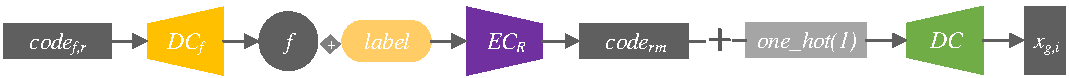
\includegraphics[width=0.98\columnwidth]{figures/make_data}
	\caption{construction of synthetic datasets.}
	\label{make_data}
\end{figure}

Due to the influence of the operation that removing tumor information during training, there are some structural feature maps with poor quality that brain contour is not closed, so we design a structural feature map filtering algorithm for this. First, we use the generator to generate a structural feature map and its corresponding mask. We perform Gaussian blur\cite{92wink2004denoising} on the structural feature map , and then use the contour search algorithm and filling algorithm provided by OpenCV to obtain all the closed contours of the Gaussian blur image and fill them. So we get a mask by the traditional algorithm, and finally we calculate the Mean Absolute Error (MAE) of the two masks. If the MAE is lower than the threshold we set, the main brain contour of the structural feature map is relatively complete, and the feature map can be used; otherwise, the main brain contour of the structural feature map is defective, the mask obtained by the traditional algorithm is hollow inside and quite different with the mask generated by the generator, so it needs to be regenerated. The algorithm is expressed as follows:
\begin{algorithm}
	\caption{Structural feature map filtering}
	\label{alg:3}
	\begin{algorithmic}[1]
		\State \textbf{function} $GetMaskFromF(img)$
		\State \indent$contours = OpenCV.findContours(img)$
		\State \indent$img =OpenCV.drawContours(img,contours)$
		\State \indent\textbf{return} $img$
		\State \textbf{end function}
		\State
		\State $mae=0.05$
		\State \textbf{do} 
		\State \indent$f, m = Generator()$
		\State \indent$m'= GetMaskFromF(f)$
		\State \textbf{while} $MAE(m',m) <= mae$
	\end{algorithmic}  
\end{algorithm}

In the multimodal MRI obtained from the selected structural feature map and matched lesion label, there are also samples with poor lesion generation. At this point, we segment our synthetic MRI data through a pre-trained lesion segmentor, the segmentation result is then evaluated with the input lesion label for the dice score, and the sample with the score above the set threshold (default 0.95) can be filtered.

After multiple filtering, we obtain the final synthetic dataset consisting of random structural feature maps, paired masks, random lesion segmentation labels, and multimodal MRI. We require that the segmented and filtered dataset can achieve a score of 0.98 or more on the segmentor trained on real data before it can be used in the data availability verification experiment.

\subsection{Training of lesion segmentation}
\begin{figure}
	\centering
	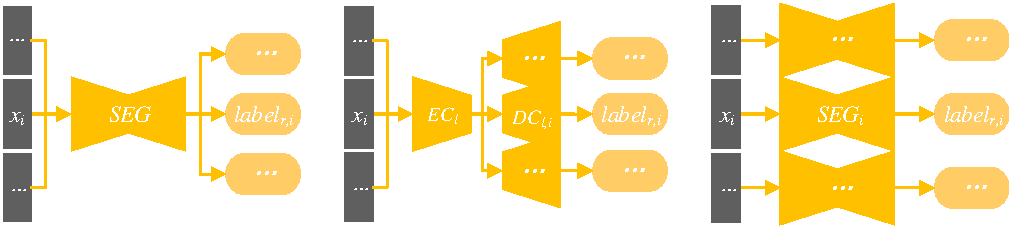
\includegraphics[width=0.45\columnwidth]{figures/segmentation}
	\caption{lesion segmentation.}
	\label{segmentation}
\end{figure}

Our lesion segmentation training process is shown in Fig. In order to verify whether the lesion data in the synthetic data is consistent with the random input lesion label, we use real data to train an independent lesion segmentor for each modality, and perform segmentation ability test on real datasets. The trained segmenter is then used to segment the image in the synthetic dataset, and the segmentation result is compared with the input lesion label to verify that the synthetic image contains the expected lesion information. In addition, we also use a data set constructed from synthetic data and real data of different data volumes to train the lesion segmentor. After training, the segmentation ability test is performed on real test dataset to verify the availability of  synthetic data.

The loss item of the segmentation training is as follows, where $label_{r,i}$ represents lesion label generated by the lesion segmentor from $x_i$
\begin{center}
		$loss_{l}=\sum\limits_{i=0}\Vert{label_i-label_{r,i}}\Vert_{2}^{2}$
\end{center}


\section{Experiments}

\subsection{BRATS2015 dataset}
We use the open dataset BRATS2015 for experiments, which has four registered modalities of T1/T2/T1c/Flair. The training dataset contains 274 3D MRIs per modality, with the size of 155$\times$240$\times$240, and 274 tumor segmentation labels of the same size. We divide the sample into a training set and a testing set by 9:1, and construct a 2D data set from 50 slices of each 55-105 of the 3D MRI. In data preprocessing, we standardized each image.

\subsection{BRATS synthetic dataset}
We constructed a registered synthetic dataset with tumor labels containing four modalities of T1, T2, T1c, and Flair using the method in ~\ref{make dataset}. The size of the synthetic dataset sample is consistent with the BRATS2015 dataset, but the number of samples can be any number according to the needs of the experiment.

\subsection{BRATS Enhanced dataset}
We performed random scaling, rotation, translation, flipping, etc. on the original BRATS2015 dataset to obtain enhanced data. The size of the enhanced dataset sample is consistent with the BRATS2015 dataset, but the number of samples can be any number according to the needs of the experiment.

\subsection{Training settings}
The number of iterations of each experiment is equal to 100 epochs of the BRATS2015 training dataset. The learning rate is 1e-4 without weight decay.  we use Adam optimizer with beta1 of 0.5 and perform a Dropout of 0.1 on the input layer, Batch size is 1. In generator components, the mean kernel filter parameter is used to initialize the convolution kernel parameter. Specifically, for a convolutional layer with a convolution kernel size of $[k,k,f]$, we initialize the $k\times k\times f$ convolution kernel parameters of this layer to $1/(k \times k\times f)$, and the bias is 0. In discriminator, we use a random normal initializer with mean of 0 and standard deviation of 0.2, and the bias is 0. We used Dice Score \cite{95dice1945measures} and Mean Square Error (MSE)\cite{94prasad1990the} to evaluate the segmentation results. The evaluation results are the average of the evaluation results of the 2D images, and each experiment is trained four times to retain the best results.

\subsection{Contrast experiment of lesion generation method}
\label{label gen methods tests}
We used the training set of the processed BRATS2015 dataset to fully train the lesion segmentor for the same iteration step, and then we selected the test set of the BRATS2015 dataset and  the unfiltered synthetic dataset by segmentor from different lesion generation component methods. Except for the difference in the source of the test data, other conditions such as the sample size of the test data are identical. Among them, the segmentation method we adopt on the real data is the multiple segmentors method in the section~\ref{label gen methods}, that is, each modality trains a separate segmentor.

\subsection{verification experiment of Synthetic data availability}
As shown in the table, we mixed real BRATS2015 training data with BRATS synthetic data in different amounts, then used the mixed data set for segmentation training, and finally evaluated the segmentation ability of the model on real BRATS2015 test data. All experiments were fully trained with the same number of iterations. Except for the difference in the source of the training data, other conditions such as the sample size of the test data are identical. At the same time, as a comparison, we also conduct a separate training of synthetic data, mixed training of real data and normal enhancement data. We set up three data mixing modes: random mixing, real first, and synthetic
first.

\section{Results}
\subsection{Quantitative result}

\subsubsection{Lesion segmentation result}
\begin{table}[t]
	\caption{Lesion segmentation result}\smallskip
	\centering
	\resizebox{.8\columnwidth}{!}{		
		\smallskip\begin{tabular}{llll}		
			\toprule	
			synthetic method&test data type &MSE   &Dice Score \\	
			\midrule		
			-&real 		   				&0.026 &0.915 \\					
			1SEG&synthetic     			&0.053 &0.741 \\			
			1ECL+4DCL&synthetic     	&0.055 &0.808 \\		
			4SEG&synthetic     			&0.043 &0.838 \\
			\bottomrule			
		\end{tabular}	
	}	
	\label{label_test}	
\end{table}

As shown in the table ~\ref{label_test}, after the BRATS2015 training data is fully trained by the same iteration step, the segmentation test results reach the MSE of 0.026 and the Dice Score of 0.915 on the real test data set. Then we use this excellent segmentor to segment our unfiltered synthetic data. On the synthetic dataset with the same amount of data as the real test dataset, three different lesion label generation component methods have achieved good segmentation results. As a result, the method in which each modality trains a separate segmentor achieves the best results, and the Dice Score also reaches 0.838.

\subsubsection{Verification experiment results for synthetic data availability}
\begin{table}[t]
	\caption{Verification experiment results for synthetic data availability}\smallskip
	\centering
	\resizebox{.95\columnwidth}{!}{
		\smallskip\begin{tabular}{lllllll}
			\toprule
			Num &real data &synthetic data & Enhanced data  & mixing modes  & MSE &Dice Score\\
			\midrule
			1& 15070 & 0  &0 &- &0.026 &0.915 \\
			31& 15070$\times$ 0.5 & 0  &0 &- &0.032 &0.902 \\
			
			2& 0 & 15070  &0 &- &0.205 &0.708 \\
			3& 0 & 15070$\times$ 2  &0 &random mixing &0.206 &0.736 \\
			4& 0 & 15070$\times$ 3  &0 &random mixing &0.205 &0.754 \\
			
			7& 15070$\times$ 0.1 & 15070  &0 &synthetic
			first &0.031 &0.908 \\
			8& 15070$\times$ 0.1 & 15070$\times$ 2  &0 &synthetic
			first &0.028 &0.907 \\
			9& 15070$\times$ 0.1 & 15070$\times$ 3  &0 &synthetic
			first &0.030 &0.907 \\	
			
			13& 15070$\times$ 0.2 & 15070$\times$ 0.8 &0  &random mixing &0.041 &0.850 \\
			12& 15070$\times$ 0.5 & 15070$\times$ 0.5 &0  &random mixing &0.031 &0.904 \\
			14& 15070$\times$ 0.8 & 15070$\times$ 0.2 &0  &random mixing &0.024 &0.935 \\
			
			32& 15070 & 15070$\times$ 0.2 &0  &random mixing &0.025 &0.921 \\
			33& 15070 & 15070$\times$ 0.5 &0  &random mixing &0.023 &0.939 \\
			34& 15070 & 15070$\times$ 0.8 &0  &random mixing &0.026 &0.916 \\
			15& 15070 & 15070 &0            &random mixing &0.027 &0.913 \\
			18& 15070 & 15070$\times$ 2  &0 &random mixing &0.033 &0.901 \\
			19& 15070 & 15070$\times$ 3  &0 &random mixing &0.034 &0.897 \\
			
			35& 15070 &0 & 15070$\times$ 0.2   &random mixing &0.027 &0.911 \\
			36& 15070 &0 & 15070$\times$ 0.5   &random mixing &0.025 &0.927 \\
			37& 15070 &0 & 15070$\times$ 0.8   &random mixing &0.026 &0.920 \\
			22& 15070 &0 & 15070           &random mixing &0.026 &0.915 \\
			23& 15070 &0 & 15070$\times$ 2 &random mixing &0.032 &0.898 \\
			24& 15070 &0 & 15070$\times$ 3 &random mixing &0.036 &0.885 \\
			
			16& 15070 & 15070 &0  &real first &0.195 &0.795 \\
			17& 15070 & 15070 &0  &synthetic
			first &0.021 &0.940 \\
			\bottomrule
		\end{tabular}
	}
	\label{use_test}
\end{table}
【TO DO】As shown in table ~\ref{use_test}, we have been trained on data sets with different components and quantities and then evaluated on real test sets to get the results in the table.In experiment 1, after the full training of 100 epochs of BRATS2015 training data, the segmentation test results reached 0.026 MSE and 0.915 Dice Score on the real test data set.According to the training results of experiment 2-4 using synthetic data alone in the table, there is still a certain gap between the training results of the synthetic data and the real data, which indicates that the synthetic data cannot completely replace the real data as the training set.The results of experiment 7-9 show that pre-training with a large amount of synthetic data and fine-tuning on a small amount of real data can achieve a result very close to that of training with real data in experiment 1. This indicates that the synthesized data is very suitable as a pre-training data set.Experiment 12-14 a percentage of the real data and synthetic data random mixing proportion of different result difference is very big, when both scale similar segmentation result with experiment 1 were similar, synthesis of high data rate, the result is lower than the experiment 1, synthetic data rate is low, can provide the generalization ability of the model, obtained is higher than the result of experiment 1.Experiment a further attempt to 32-34, 18th - 19 in the total amount of real data synthesis data of adding different amount of data, we found that fewer synthetic data can improve the generalization ability of the model, have the effect of data enhancement, synthetic data enhancement effect, the better, the more but when synthetic data to increase again after a certain proportion will have the opposite effect, the synthetic data, the more the influence of the real data.Experiment 35 to 37 and 22 to 24, we use the enhancement data generated by a data enhancement method to enhancement effect compared with the synthetic data, we found the data volume increased and enhanced effect on the change tendency of the two is consistent, but the difference in specific enhancement effect as the change of enhanced data volume change curve there are some differences. Overall, in terms of the sensitivity of the model to the amount of enhanced data, the enhanced data is more robust, but the upper limit of the enhancement effect that can be achieved by the composite data is much higher than that of the former strong data.In experiment 16-17, we compared experiment 15 and found that the synthesized data with the same amount of real data had the best performance as pre-training data before real data training, the mixed training effect as enhanced data and real data was in the middle, and the training performance after real data set as supplementary training data was very poor.

【TO DO】AsIn general, we find that when the amount of real data is large, a small amount of composite data can be used as mixed enhancement data, or a large amount of composite data can be used for pre-training before training on real data sets. When real data is scarce, large amounts of synthetic data can be used for pre-training, and then fine-tuned on a small amount of real data to obtain results that compete with the training of completely real data. This is consistent with the conclusion of \cite{4shin2018medical}. We do not recommend full use of synthetic data for training, and contrary to the conclusion of \cite{4shin2018medical}, we do not recommend supplementary training using synthetic data either.

\subsection{Synthetic images}
【TO DO】AsFigure ~\ref{generated_f} shows an example of the structural feature graph we generated from the random normal distribution matrix. In figure ~\ref{generated_mri}, we show several examples of structural feature maps generated from random normal distribution matrices, corresponding masks generated from structural feature maps, randomly selected lesion segmentation labels, and multi-modal MRI generated from structural feature maps and lesion segmentation labels.
\begin{figure}
	\centering
	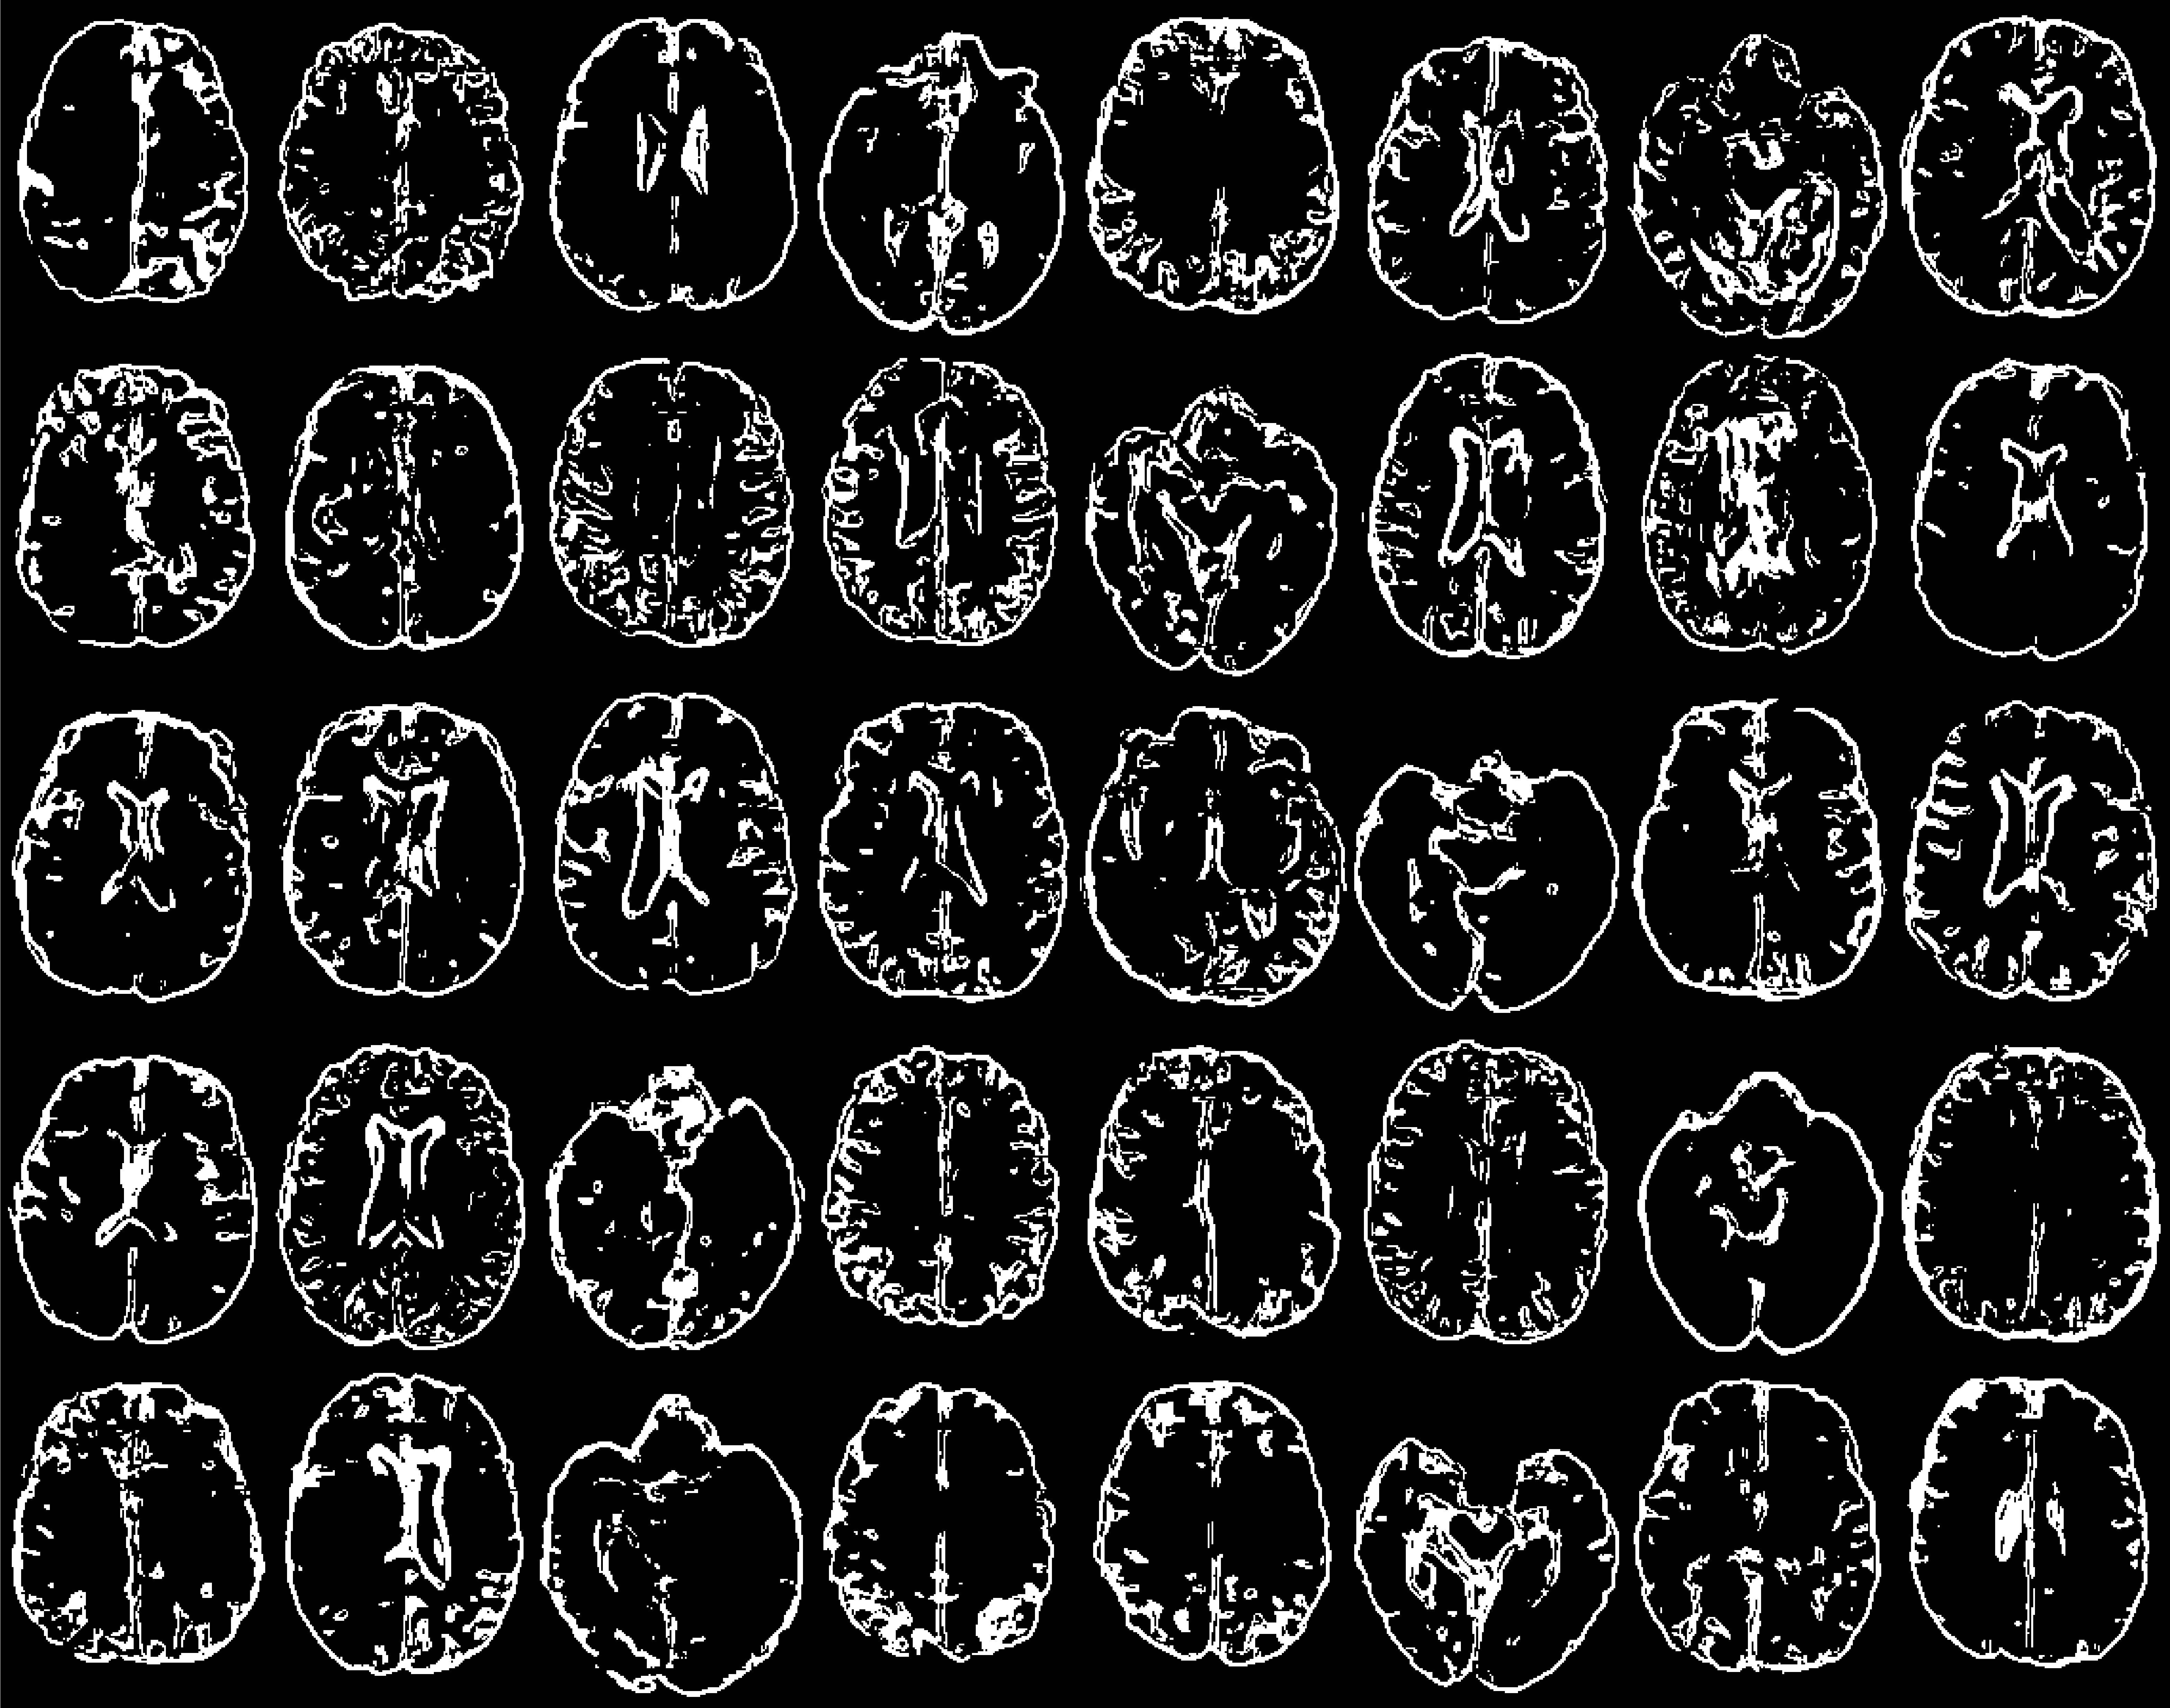
\includegraphics[width=0.8\linewidth]{figures/Fs}
	\caption{Synthetic structural feature map.}
	\label{generated_f}
\end{figure}

\begin{figure}
	\centering
	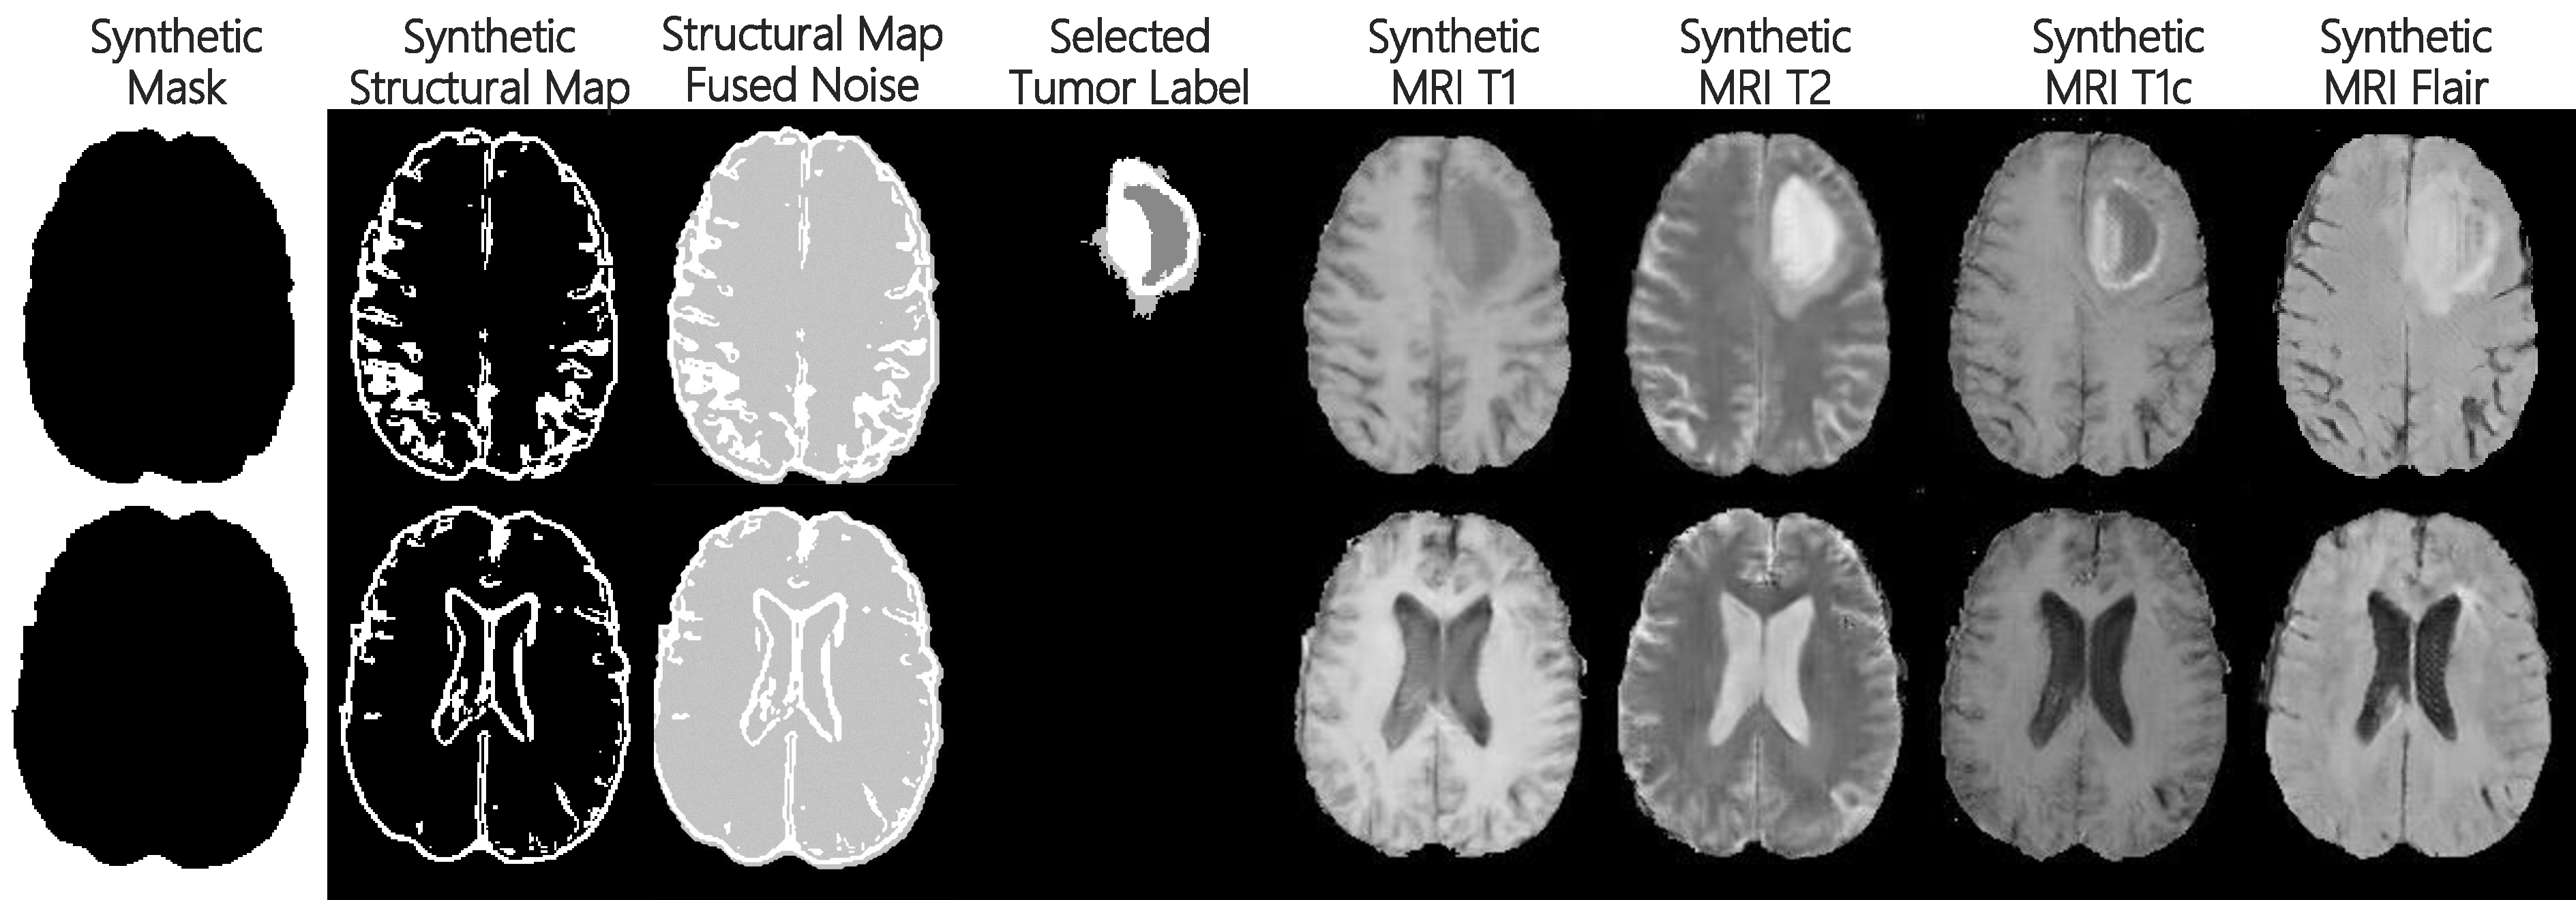
\includegraphics[width=0.75\linewidth]{figures/F_to_MRI}
	\caption{Multimodal MRI generated from the random structural feature map and lesion label.}
	\label{generated_mri}
\end{figure}

\section{Conclusion and future work}
Based on the conditional generation antagonism network, we realized the generation of registered multimodal MRI from the random normal distribution matrix through unsupervised training, and could add the lesion information freely. 
We verified through lesion segmentation experiments that synthetic MRI can be used as pre-training data or enhanced data for intelligent medical image processing tasks and can significantly improve the generalization ability of the model.
In this paper, our contributions include the following:
\begin{itemize}
	\item We propose a structural feature map extraction method to extract anatomical structure information directly from medical images without training or additional label data;
	\item We propose a random structure feature map generation method to generate structural feature maps from multi-dimensional normal distribution sampling;
	\item We realized the generation of registered multimodal MRI with corresponding lesion information from structural feature map and randomly selected lesion labels;
	\item We verified that synthetic data can be used as pre-training data or enhanced data for intelligent medical image processing tasks through a number of data usability tests on our synthetic dataset.
	
\end{itemize}

In the future, we will further improve our method in CT, PET and other modes, in heart, lung and other parts, in detection, classification and other lesion processing tasks. We are committed to further simplifying the training process and synthesizing higher quality medical images.	

\section{ Acknowledgments}

Thanks for the computing support provided by NSCCGZ.


\bibliography{refer}
\bibliographystyle{aaai}

\end{document}
